\chapter{Two ledgers and the virial balance}\label{ch:ledgers}

\section{The old idea}

An old intuition holds that stable things are balanced things: when one side gains, another gives, and what persists is
what the balance allows. In mechanics the intuition has a precise form, the virial theorem. Chapter~\ref{ch:virial_law} treats it
as one application of IAM's Law, the one that sets how much bound matter writes, not as its basis. This chapter states
what the theorem says exactly, where a genuine one half appears in physics, and what carries over to the cell.

\section{What the virial theorem says}

For a bound system in a steady state whose potential energy is a homogeneous function of degree $k$
in the coordinates, $U\propto r^k$, the time averages of kinetic and potential energy satisfy
\begin{equation}
  2\langle K\rangle=k\,\langle U\rangle .
  \label{eq:virial}
\end{equation}
\derived{} For gravity and electrostatics, $k=-1$, so $2K+U=0$: $U=-2K$ and the total energy is
$E=K+U=-K=U/2$ (Figure~\ref{fig:partition}a). The theorem does not say that kinetic and potential
energy are equal. It says the potential energy is twice the kinetic in magnitude and opposite in sign.
For a harmonic potential, $k=2$, and $K=U$; for a linear (confining) potential, $k=1$, and $2K=U$.

\begin{figure}[htbp]\centering
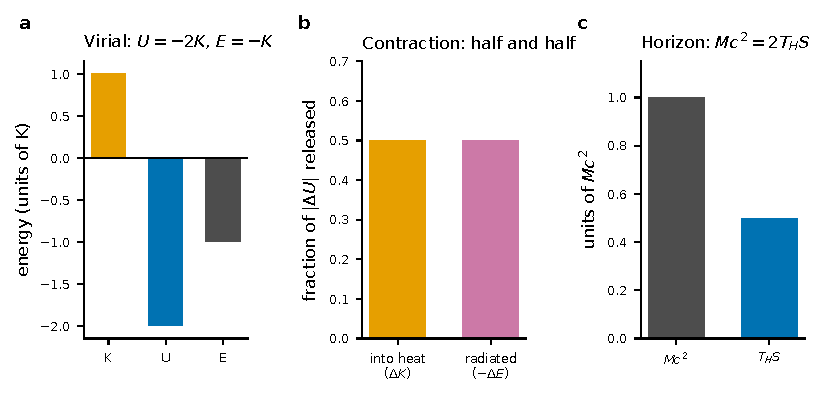
\includegraphics[width=\textwidth]{figures/part6/fig_energy_partition.pdf}
\caption{Three statements about energy that are often run together. (a) The virial theorem for an
inverse-square force. (b) The energy released when a self-gravitating body contracts slowly: half
goes into heat, half is radiated. (c) The Smarr relation for a Schwarzschild black hole. \derived}
\label{fig:partition}
\end{figure}

\section{Where the halves really are}

Three exact results do contain a factor of one half, and they are the content behind ``half and
half''.

\paragraph{Contraction.} When a self-gravitating body contracts quasi-statically, $U$ becomes more
negative by $|\Delta U|$. Since $E=U/2$, the total energy falls by $|\Delta U|/2$, which is radiated,
and $K=-E$ rises by $|\Delta U|/2$, which heats the body (Figure~\ref{fig:partition}b). Half of the
released potential energy is kept as heat and half leaves as light. This is why a contracting
protostar heats up as it loses energy, and it is the Kelvin--Helmholtz mechanism. \derived

\paragraph{The horizon.} For a Schwarzschild black hole of mass $M$, the Hawking temperature
$T_H=\hbar c^3/8\pi GM\kB$ and the entropy $S=4\pi GM^2\kB/\hbar c$ satisfy
\begin{equation}
  Mc^2=2\,T_HS ,
  \label{eq:smarr}
\end{equation}
the Smarr relation~\cite{Smarr1973} (Figure~\ref{fig:partition}c). Evaluated for one solar mass,
$T_HS=8.94\times10^{46}$~J and $Mc^2/2=8.94\times10^{46}$~J. \calc{} The horizon's thermal energy,
the Landauer cost of every bit it holds at its own temperature, is exactly half its mass-energy.

\paragraph{Atoms, molecules and cells.} Every atom and every chemical bond is held by electromagnetism, a $1/r$ potential, so the
virial half holds inside every molecule of a cell exactly as it holds for a star: for an atom or molecule at its equilibrium
geometry the quantum virial theorem gives $2\langle K\rangle=-\langle V\rangle$. For hydrogen in its ground state $\langle K\rangle=13.6$~eV and
$\langle V\rangle=-27.2$~eV. \derived{} The DNA, the enzymes that copy its marks and the ATP that pays for them are all
bound this way.

\paragraph{Switching a transistor.} Charging a capacitance $C$ to voltage $V$ from a fixed supply draws $CV^2$ from the supply; $\tfrac12CV^2$
is stored and $\tfrac12CV^2$ is dissipated in the resistance, whatever its value; the stored half is dissipated when the node discharges.
\derived{} Every CMOS write therefore splits its energy in halves. Whether this half and the virial half are one statement of IAM's Law is
open. \conjecture

\paragraph{Equipartition.} In thermal equilibrium each quadratic degree of freedom holds $\kB T/2$.
This is a different half: a statement about how energy is shared among degrees of freedom, not about
kinetic versus potential energy.

\section{The two ledgers}

IAM keeps two accounts for every system (Chapter~\ref{ch:iams_law}).
\begin{description}
\item[The geometric ledger] is the capacity of the encoding surface: area over $4\lP^2$ for a
      horizon, one bit per CpG copy for a methylome.
\item[The information ledger] is what has been committed to that surface: the running total of
      irreversible events, each charged at least $\kB T\ln2$ at the surface's temperature.
\end{description}
In cosmology the information ledger enters Jacobson's entropy functional as an informational term; the partition
coefficient $\beta_m=\Omega_m/2$ that sets its size follows from the virial statement. Both are treated and labeled in
Chapters~\ref{ch:virial} and~\ref{ch:theory}. \conjecture

\section{What carries over to the cell}

IAM's Law operates in the cell as it does everywhere: every mark written or lost is an irreversible event charged at least
$\kB T\ln2$ at 310~K (Chapter~\ref{ch:landauer}), and the virial half holds for every molecule the cell is built of. One further
picture offered for the cell is that, like a star, it pays for its irreversible work in two halves: one half as metabolism (the work,
the heat, the activity) and one half written into the methylation pattern.

\begin{keybox}[title=Status of the two-halves picture for a cell]
The picture is \conjecture. No experiment in the literature or in this instrument measures the
partition of a cell's free-energy dissipation between ``motion'' and ``record'', and the numbers of
Chapter~\ref{ch:landauer} show that methylation maintenance is a very small part of the cell's energy
budget (of order $10^{-7}$). If there is a partition, it is not of the cell's total energy. It could
be of something narrower, for example of the free energy dissipated per write at the maintenance
machinery, but no such quantity has been defined and measured. \openprob

Nothing in the Cellular Performance Gauge uses the partition. The gauge reads the information ledger
directly, as entropy on the identity sites or copy error on single molecules, and compares it with the same cell type's
healthy reading. It would read the same if the
two-halves picture were wrong.
\end{keybox}

What does carry over exactly is the logic of Eq.~\eqref{eq:smarr}: for any encoding surface, the
Landauer cost of what it holds, at its own temperature, is a physical quantity with a definite value.
For a cell's methylome of $\sim2.8\times10^7$ bits at 310~K, the cost of holding its capacity is
$8.4\times10^{-14}$~J. \calc{} That is the cellular entry in the ledger, and it is small because both
the temperature and the bit count are small compared with a horizon's product.

Table~\ref{tab:p4_halves} collects the halves of this chapter with their values. Figure~\ref{fig:p4_ledger} places the cell's ledger entry
beside the horizons'. For a Schwarzschild horizon the cost of holding its capacity at its own temperature, $N\kB T_H\ln2=T_HS$, is half the
mass-energy at every mass. The cell's entry, $8.4\times10^{-14}$~J, carries no such relation to anything the cell is made of. \calc

\begin{figure}[htbp]\centering
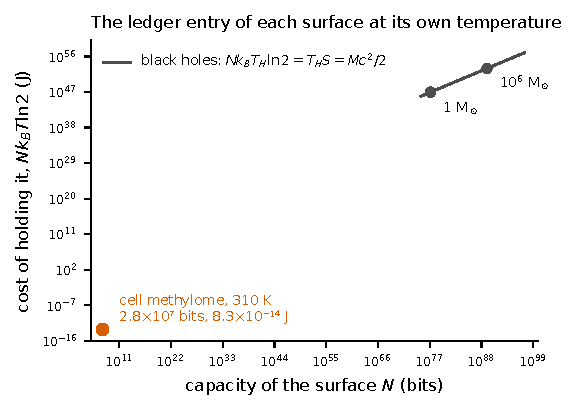
\includegraphics[width=0.62\textwidth]{figures/part6/fig_p4_04_ledger.pdf}
\caption{The ledger entry of three surfaces: capacity $N$ against the cost of holding it, $N\kB T\ln2$, at the surface's own temperature. The line is
the Schwarzschild family, on which the entry equals $Mc^2/2$ (one solar mass: $T_HS=8.94\times10^{46}$~J). The cell: $2.8\times10^7$ bits at 310.15~K.
\calc{} (CODATA constants).}
\label{fig:p4_ledger}
\end{figure}
\begin{table}[htbp]\centering\small
\caption{Where a factor of one half appears, and what it splits. \calc{} values from CODATA constants.}\label{tab:p4_halves}
\begin{tabular}{@{}p{0.27\textwidth}p{0.17\textwidth}p{0.33\textwidth}l@{}}\toprule
system & relation & the half & status \\\midrule
hydrogen, ground state & $2\langle K\rangle=-\langle V\rangle$ & $\langle K\rangle=13.61$ eV, $\langle V\rangle=-27.21$ eV & \derived \\
slow contraction of a self-gravitating body & $E=U/2$ & half of $|\Delta U|$ heats, half is radiated & \derived \\
charging a capacitance from a fixed supply & drawn $CV^2$ & $\tfrac12CV^2$ stored, $\tfrac12CV^2$ dissipated & \derived \\
Schwarzschild horizon, one solar mass & $Mc^2=2T_HS$ & $T_HS=8.94\times10^{46}$ J; $Mc^2/2=8.94\times10^{46}$ J & \calc \\
equipartition, 310.15 K & $\tfrac12\kB T$ per quadratic term & $2.14\times10^{-21}$ J (a different half) & \derived \\
\bottomrule
\end{tabular}
\end{table}

\section{What the balance is for}

The value of the balance is that it directs attention to budgets and to what happens when a system is driven past what its
surface can hold. On a horizon that is saturation. On a cell it is the subject of the next chapter.
